\section{Materiales y métodos}

\subsection{Limpieza del Material de Vidrio}
El material de vidrio empleado para la síntesis de nanopartículas debe ser limpiado exhaustivamente. Todo el material se sumerge en solución saturada de permanganato de potasio (\ce{KMnO4}) en medio alcalino. Se calienta a ebullición por 2h y se deja enfriar. Posteriormente se enjuaga parcialmente con agua ultra-pura y se remueve el deposito de dióxido de manganeso (\ce{MnO2}) con agua oxigenada diluida en medio ácido. Por último se enjuaga copiosamente con agua ultra-pura y se seca en estufa. Este procedimiento remueve los restos de ``grasa'' o materia orgánica en la superficie del vidrio. El usar un oxidante muy fuerte como el \ce{KMnO4}, la materia orgánica pasa a \ce{CO2}. También se empleó ``solución piraña'' (\ce{H2SO4}:\ce{H2O2}; 3:1) por \qty{5}{\minute} seguido de enjuague copioso con agua ultra-pura para remover materia orgánica de pipetas, probetas (material volumétrico que no puede calentarse).

Para remover restos de metales de la superficie de vidrio, el material fue lavado con ``agua regia'' (\ce{HCl}:\ce{HNO3}, 3:1), seguido de enjuague con agua ultra-pura.

\subsection{Síntesis de las nanopartículas}
%Síntesis de las nanopartículas
%\textbf{Síntesis.}. 
Las nanopartículas fueron sintetizadas siguiendo el proceso descrito por Zhang (2011)\cite{zhang2011}. 
El volumen total de la solución es fijado en \qty{25}{\milli\liter}.
Se disuelve nitrato de plata (\ce{AgNO3}, \qty{50}{\milli M}, \qty{50}{\micro\liter}), citrato de sodio (\ce{Na3C6H5O7}, \qty{75}{\milli M}, \qty{75}{\milli M}) y peróxido de hidrógeno (\ce{H2O2}, \qty{30}{wt\percent}, \qty{60}{\micro\liter}) en \qty{24.75}{\milli\liter} de agua ultra pura (\SI{18}{\mega\ohm}).
Luego se añade borohidruro de sodio (\ce{NaBH4}, \qty{100}{mM}, \qty{250}{\micro L}) a la solución bajo agitación.
Inmediatamente tornándose de un color amarillo claro. 
Unos minutos después la solución cambia a amarillo oscuro, rojo, verde y azul sucesivamente.
En función de las proporciones utilizadas la reacción es detenida en cualquier color intermedio.

En la sección \ref{SEC:mecanismo_formacion_particulas_triangulares} se describe en rol de cada reactivo en la formación de las AgNPs.

\subsection{Caracterización de las nanopartículas.}

\subsubsection{Microscopio electrónico de transmisión}
%TODO: Seguir el orden que usa Gastón para explicar el funcionamiento del TEM. Por ahí profundizar un poco más. 
% No hace falta que todo sea seco, hay que meterle un poco de varieté

% Esquema sacado de la tesis doctoral de Gastón Corthey 2012
\begin{figure}[h]
	\centering
	
\includegraphics[width=0.7\linewidth]{./TEM/esquema_TEM_tesis}
	\caption{Esquema de un microscopio electrónico de transmisión (TEM) convencional con cañón de electrones de emisión termoiónica de LaB6 \cite{corthey2012}. } 
	\label{fig:esquematemtesis}
\end{figure}

% Funcionamiento general del microscopio
% TODO: Mencionamos algo del límite de información? Una ecuación salvaje por ahí...
Para observar una nanopartícula es necesario disponer de un dispositivo que tenga resolución nanométrica, lo que está fuera del alcance de cualquier microscopio óptico.
Además, a esta escala la mayoría de microscopios electrónicos comienzan a tener dificultades.
Sin embargo, los microscopios electrónicos de transmisión (TEM) se adecúan bien al análisis de nanopartículas.
Las muestras de TEM deben ser extremadamente delgadas y el pequeño tamaño de las partículas, que podría ser inconveniente en otro sistema, las vuelve ideales para el método.

En microscopia electrónica de transmisión se incide sobre una muestra con un electrones de alta energía y se observan los transmitidos. La técnica es ampliamente versátil, permitiendo estudiar morfología, estructura cristalina y propiedades químicas utilizando un solo equipo. 

Todos los sistemas de funcionamiento del microscopio están alojados dentro de una columna vertical, Fig. \ref{fig:esquematemtesis}. Se agrupan en 5 sistemas principales; sistema de vacío, cañón de electrones, portamuestras, sistema de lentes y pantalla/cámara.

% Sistema de vacio - altas tensiones - iteracción electrones muestra
% TODO: Qué cañones de electrones necesitan estar a una presión menor?
Para que el haz de electrones alcance la muestra es necesario asegurarse que en todo el recorrido hasta la muestra no interaccione con ninguna molécula. Para lograrlo la columna del microscopio se mantiene en ultra alto vacío, \(\sim 10^{-7} \, \si{Torr}\). Además, ciertos cañones de electrones, por generar un potencial alto y confinado, tiene que estar a una presión aún menor para funcionar correctamente. El vacío se genera utilizando una bomba mecánica para vaciar a altas presiones, una difusora para alcanzar alto vacío y una bomba de ionización por llegar al ultra alto vacío.

% Cañón de electrones
% TODO: Explicar un poco cada mecanismo y las ventajas y desventajas de este
% Daño por knock-on or knock off
El cañón de electrones se encarga de generar el haz. Existen diferentes en función del mecanismo de emisión; cable de Tungsteno, cristal de \ce{LaB6} y FEG. Estos se diferencian por el tamaño del haz, la intensidad máxima y la dispersión de energía. Una vez desprendidos, los electrones son acelerados por una potencial electrostático de \(\sim \SI{100}{\kilo \volt}\), cuyo valor determina la longitud de onda de los electrones emitidos. Así como también controla el daño por \textit{knock-on} que va a sufrir la muestra. 

% 	-- Porta muestras --
%TODO: Mejorar la notación - frente - espalda es muy ambígüo. Por ahí buscar algo similar a superior e inferior o distinguir por funcionalidad
%TODO: Agregar escala a la imágen del portamuestras, no hace falta que sea demasiado correcta
%TODO: Agregar una imágen del portamuestras entero al costado que se vea todo el sistema a lo largo.
\begin{figure}
	\centering
	\begin{subfigure}{0.7\columnwidth}
		\centering
		
\includegraphics[width=\textwidth]{porta_muestra/frente.JPG}
		\caption{Frente}
	\end{subfigure}
	
	\begin{subfigure}{0.7\columnwidth}
		\centering
		
\includegraphics[width=\textwidth]{porta_muestra/espalda.JPG}	
		\caption{Espalda del portamuestras}
	\end{subfigure}
	
	\caption{Imagen del portamuestras utilizado. Se observa el sistema de resorte para sostener la grilla.}
	\label{fig:portamuestras}
\end{figure}

% TODO: Redactar la preparación de la muestra, se hace en resultados o lo ponemos acá en métodos?
En el centro de la columna se encuentra el porta muestra. Hay varios diseños en función de las propiedades a medir y según como se necesita manipular el espécimen. El que se utilizó para observar las nanopartículas, Fig. \ref{fig:portamuestras}, consiste de una base circular de metal donde se apoya la grilla con muestra y una ``arandela'' que la sostiene.

% Sistema de lentes 
% Se podría agregar algo de como funciona una lente en general antes de pasar a epxlicar los diferentes roles que cumplen.
A lo largo de la columna se encuentran varias lentes de electrones. Se separan en 3 tipos por la función que cumplen; condensadoras, objetivo y proyectoras. 

\textbf{Lentes condesadoras.}
Colocadas debajo del cañón. Su labor principal es alinear el haz dentro de la columna. Con estas nos encargamos de que el haz incida de la manera que más nos convenga sobre la muestra. Y que estemos minimizando al máximo las aberraciones en la imagen resultante. Utilizan corrientes de \(\sim \SI{2}{\ampere}\).

% Por qué debía ser tan chica la distancia focal? Disminuir aberraciones?
\textbf{Lentes objetivo.}
Están luego de las condensadoras y rodean las muestra. Convergen el haz de electrones sobre la muestra. La distancia focal es chica, \(\sim \SI{5}{mm}\) y lleva a que el portamuestras se coloque directamente ``dentro'' de la lente. Para alcanzar esta distancia focal utiliza una corriente de \SI{12}{\ampere}. 

\textbf{Lentes proyectoras}
Debajo del portamuestra se encuentran la lentes que forman la imágen. Como lo indica su nombre proyectan la imagen sobre la pantalla. La mayor parte de la magnificación se realiza aquí. Utilizan corrientes de \(\sim \SI{2}{\ampere}\).

% 	-- Pantalla y cámara --
% TODO: Agregar él modelo de la cámara.
La columna posee una pantalla fluorescente para analizar las imágenes en vivo y debajo de la pantalla se coloca una cámara digital, usualmente CCD, para realizar el registro de los datos.

Ademas, se dispone de un sistema de aperturas que permiten colimar el haz/imagen en diferentes planos dentro de la columna.

% 	-- Discusión de las aberraciones y CTF --
% Cómo cito las figuras del doctorado? solo con \cite o las incluyo en el texto?
\subsubsection{Aberraciones}
\begin{figure}[h]
	\centering
	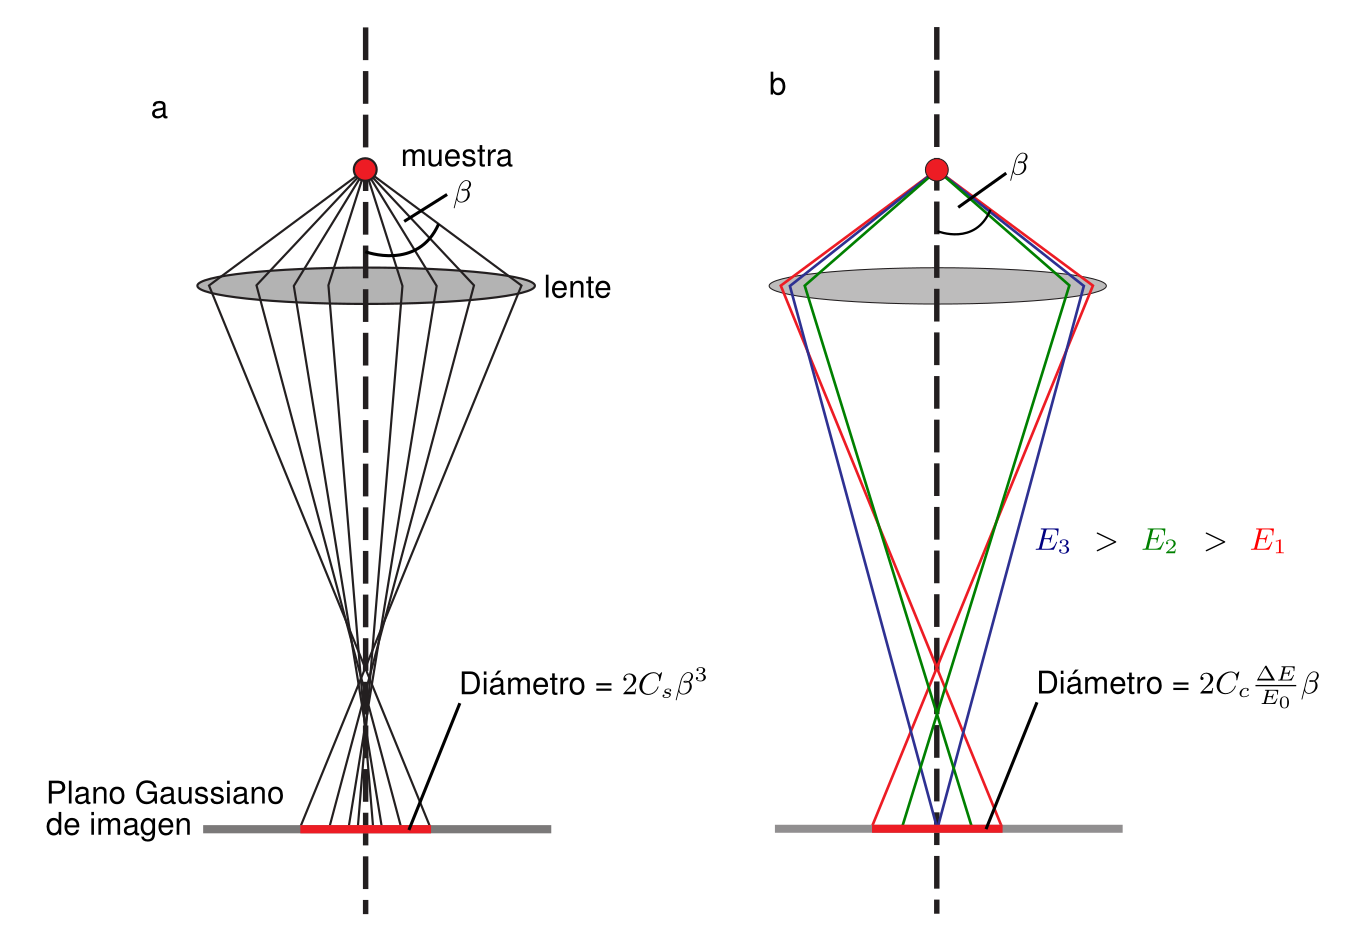
\includegraphics[width=1\linewidth]{assets/TEM/aberraciones}
	\caption{(a) Diagramas de rayos aberración esférica. (b) Diagrama de rayos aberración cromática. Diagramas tomados de la tesis doctoral de Corthey.\cite{corthey2012}}
	\label{fig:aberraciones}
\end{figure}

% Mencionar algo de microscopios corregidos
% TODO agrega la cita de que no existen las lentes divergentes. Cual libro de microscopia debería funcionar
% Ver como mencionar lo de los microscopios corregidos si es que se menciona. Decimos que son muy caros, o algo de que no están a nuestro alcance todavía?
No existen las lentes perfectas, todas presentan aberraciones de distinto tipo. Si la distancia focal varia el parámetro de impacto se le llama aberración esférica. Si la distancia focal varía con la longitud de onda se le llama aberración cromática. En un sistema óptico clásico las aberraciones son corregidas utilizando un arreglo de lentes convergentes y divergentes. Sin embargo, no se pueden fabricar lentes de electrones simétricas divergentes. Recientemente se han fabricado TEMs corregidos, que utilizan lentes asimétricas para obtener reproducir el efecto de una lente divergente y así corregir la aberración. Pero la aparición de aberraciones en TEMs clásicos es inevitable \cite{}. 

% Podría poner acá la ecuación del límite de información.
Estas aberraciones son las que finalmente ponen el límite de resolución de un microscopio de transmisión electrónica. El efecto de las aberraciones sobre la imagen final se modela utilizando la función de transferencia de contraste (CTF), que indica como se modifica cada componente de la imagen en el espacio recíproco.

% Hablar de la CTF

\subsubsection{Métodos de uso del microscopio.}
Entre las técnicas de microscopía de transmisión electrónica hay 3 que fueron de nuestro interés. Contrase de fase, amplitud e imágenes de alta resolución.

% Modos de utilización
\begin{figure}
	\centering
	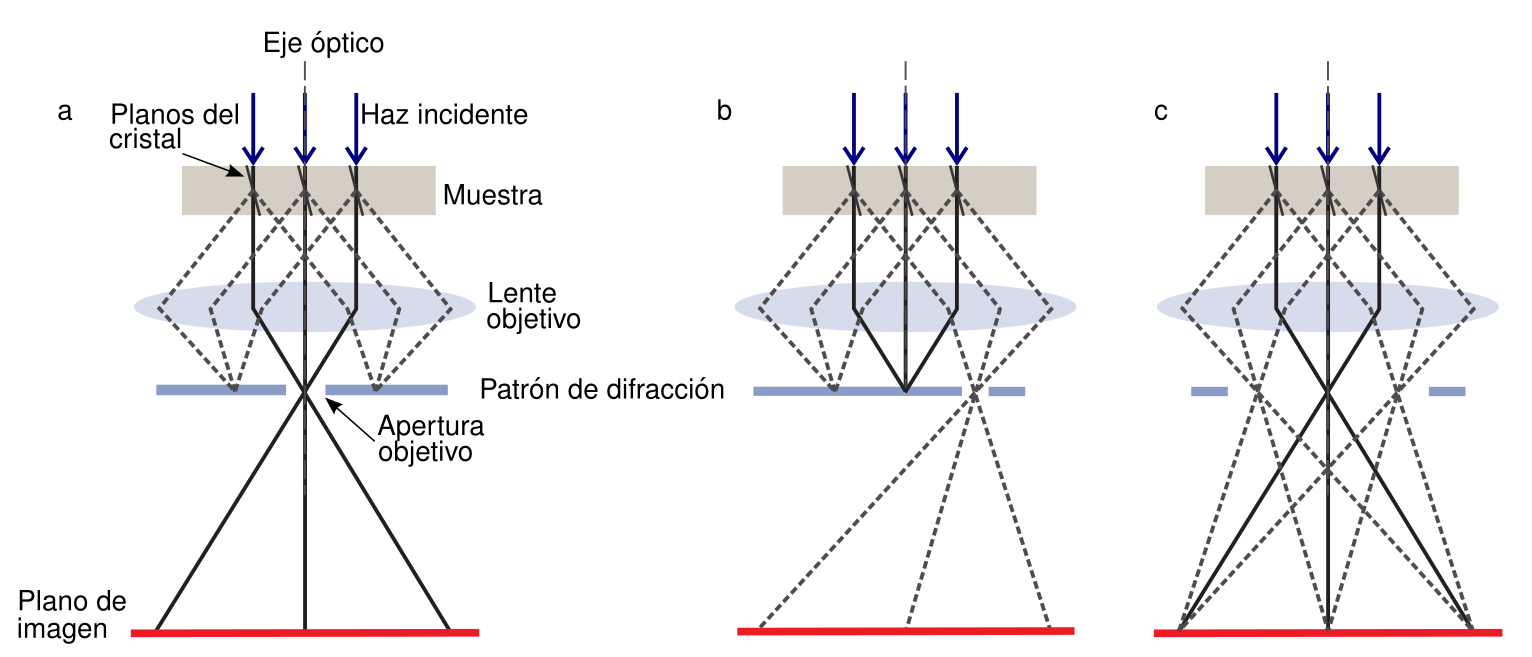
\includegraphics[width=\linewidth]{assets/TEM/modos_TEM_tesis}
	\caption{Diagrama de los diferentes modos de imagen en TEM.\cite{corthey2012} (a) Campo claro. (b) Campo oscuro. (c) Contraste de fase (HRTEM).}
	\label{fig:modostemtesis}
\end{figure}

Para caracterizar las partículas sintetizadas se utilizaron varias técnicas de microscopía de transmisión electrónica.
El objetivo principal fue utilizar microscopía de al resolución HRTEM, para obtener información de la disposición de las fallas de apilamiento dentro de la nanopartícula.
Lamentablemente, durante todo el trayecto del trabajo, ambos microscopios disponibles se encontraron bajo mantenimiento.
Por lo que solo fue posible tomar imágenes en lo que se llama campo claro y campo oscuro de las nanopartículas.

A pesar de estas complicaciones, utilizando imágenes de HRTEM tomados en el 2017, fue posible realizar un análisis integral de las imágenes mediante simulaciones de imágenes TEM.

Se utilizó un microscopio de transmisión electrónica Philips CM200. Se tomaron imágenes tanto de alta resolución (HRTEM) como en contraste de fase.

Las imágenes obtenidas mediante HRTEM son un combinación compleja de los haces de electrones difractados y transmitidos. Para analizarlas se realizaron simulaciones computacionales.

% Simulaciones
\subsubsection{Simulaciones}
Se utilizó la librería de python ABTEM y se realizaron las simulaciones en un entorno digital google colab utilizando tarjetas gŕaficas para acelerar la computación.
Las imágenes fueron simuladas utilizando el método \textit{multislice} para diferentes estructuras, sanguchitos de fcc con hcp en el centro.